\chapter{Suspensión y lazos de un espacio}
Primero veamos un tipo de espacios topológicos que nos será de gran utilidad de aquí en adelante.
\section{CW-complejos}
Un CW-complejo es un tipo particular de espacio topológico muy útil en la teoría de homotopía. Veamos su construcción: \par
Comenzamos con $X^0$ un espacio topológico discreto compuesto por las $0$-celdas. Adjuntamos $I_1$ $1$-celdas a $X^0$ para formar el $1$-esqueleto.
\[ X^1 = X^0 \cup_{f_\alpha} \left( \dot{\cup} \, e_\alpha^1 \right) \quad \alpha \in I_1\]
Inductivamente, suponemos construido el $(n-1)$-esqueleto $X^{n-1}$ al que adjuntamos una familia de $n$-celdas $\{e_\alpha^n\}_{\alpha \in I_n}$ mediante las correspondientes aplicaciones de adjunción $f_\alpha : S^{n-1} \longrightarrow X^{n-1}$. \par 
Llegado a este punto, tenemos entonces dos opciones: el proceso se detiene en un $n$, en cuyo caso la topología ya está definida, o podemos seguir indefinidamente en la sucesión
\[ X^0 \subset X^1 \subset \ldots \subset X^n \subset \ldots \]
y consideramos $\displaystyle X = \cup_{n \geq 0} X^n $ al que asignamos la topología débil heredada de los esqueletos, esto es, $A \subset X$ es abierto si y sólo si $A \cap X^n$ es abierto de $X^n$ para todo $n \geq 0$. \par 
A todo espacio $X$ así construido se le denomina CW-complejo, y se denomina CW-descomposición al conjunto de todas las celdas adjuntadas, $\xi = \{e^k_\alpha\}_{k \in \bb{N}, \ \alpha \in I_k}$. \par
Diremos que el CW-complejo es finito si el número de celdas de la CW-descompo-sición es finito. Asimismo $X$ es de dimensión finita si $X = X^n$ para algún $n \in \bb{N}$ y se denomina dimensión del CW-complejo al menor $n$ para el que ocurra ésto. \par
Si $\varphi : E^n \longhookrightarrow X \dot{\cup} e^n \longrightarrow X \cup_f e^n$ es la aplicación característica de la adjunción de una celda, llamaremos a $\varphi(E^n)$ ``celda'' y a su interior ``celda abierta''. Nótese no obstante que en un CW-complejo una ``$n$-celda abierta'' sólo es abierta en el $n$-esqueleto, pero en general no lo es en el complejo.
\begin{ejems}
\begin{itemize}
\item[(1)] Una superficie orientable compacta $M_g$ de género $g$ ($ g \geq 1$) puede ser construida a partir de un polígono de $4g$ lados identificando los lados de forma que se alternan pares de éstos. Para mayor claridad, a continuación se presentan algunos casos: \par
\begin{figure}[h]
\centering
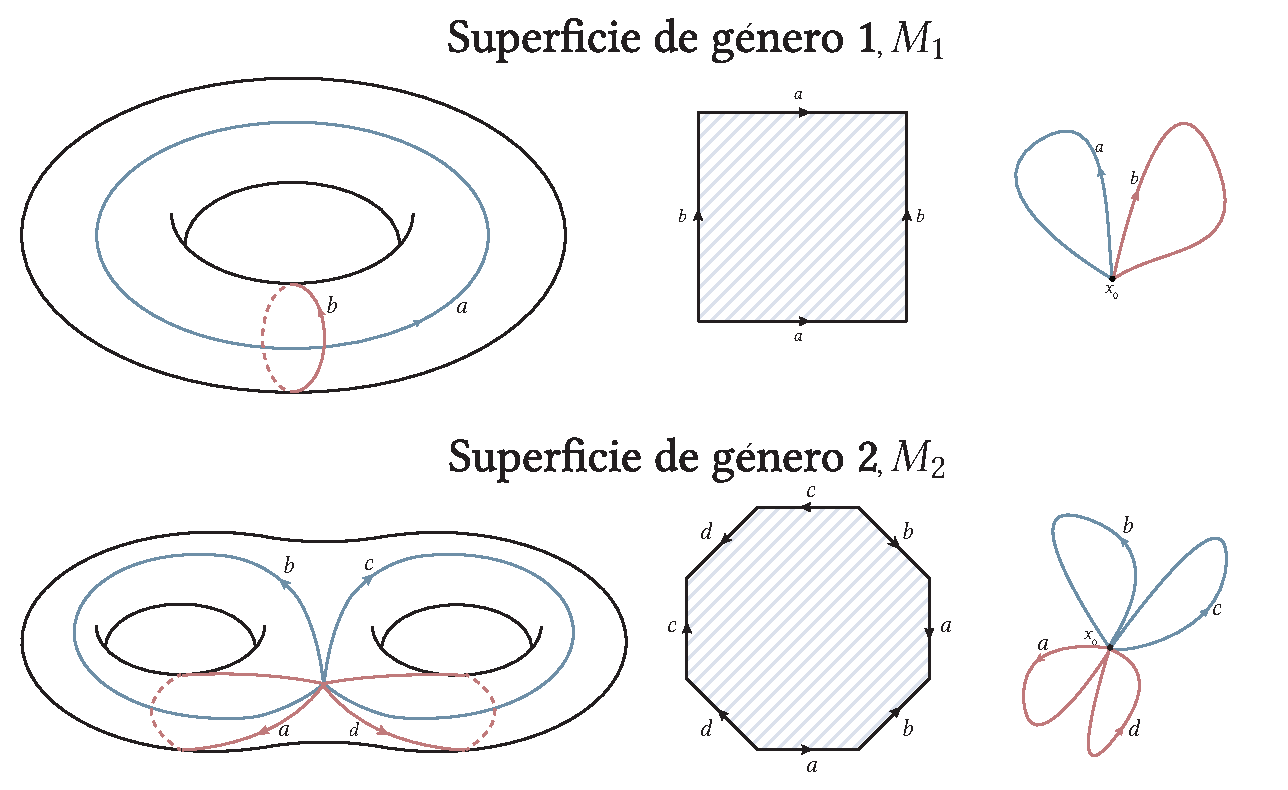
\includegraphics[width=\textwidth]{images/supgeng.pdf}
\end{figure} 
\par 
Con estas identificaciones, los $4g$ lados del polígono se transforman en $2g$ circunferencias unidas por un punto, es decir, la adjunción a $X^0 = \{ \ast \}$ de $2g$ $1$-celdas mediante la única posible aplicación de adjunción $S^0 \longrightarrow X^0$. Una vez adjuntadas estas celdas, se le adjunta una $2$-celda que es el interior de dicho polígono. \par
Así pues, $M_g = X^2$ con 
\begin{align*} 
X^0 &= \{ \ast \} \text{,  } X^1 = \bigvee_{2g} S^1 \\
M_g &= X^2 = X^1 \cup_f e^2
\end{align*}

\item La esfera $S^n$, con $n \geq 0$, tiene estructura de CW-complejo. Existen dos descomposiciones diferentes muy intuitivas: 
\begin{enumerate}
\item La primera consiste en dividir la esfera en una $0$-celda y una $n$-celda. Por ejemplo, como $0$-celda podemos tomar el polo norte $\{N\}$, y como $n$-celda tomar $S^n - \{N\}$.
\item Otra CW-descomposición consiste en comenzar con el $0$-esqueleto formado por dos puntos, esto es, $S^0$. A éstos les adjuntamos dos $1$-celdas, obteniendo $S^1$.  Y vamos adjuntando para cada dimensión $2$ $k$-celdas hasta llegar a $S^n$. Así, tendríamos una CW-descomposición formada por $2$ celdas en cada dimensión hasta la $n$-ésima.
\end{enumerate}

\item El espacio proyectivo real $\mathbb{R}P^n = \faktor{\bb{R}^{n+1}-\{0\}}{\sim}$ donde la relación $\sim$ viene dada por $x \sim y$ si $\exists \lambda \neq 0$ tal que $\lambda x = y$. La aplicación 
\begin{align*}
\bb{R}^{n+1} - \{0\} &\longrightarrow S^n \\
x &\longmapsto \frac{x}{\|x\|}
\end{align*}
induce un homeomorfismo
\[ \bb{R}P^n = \faktor{\bb{R}^{n+1} -\{0\}}{\sim} \stackrel{\cong}{\longrightarrow} \faktor{S^n}{x \sim -x} \]
Por otra parte, la inclusión de un hemisferio $S_+^n \longhookrightarrow S^n$ también induce de forma obvia un homeomorfismo $\faktor{S_+^n}{\sim} \stackrel{\cong}{\longrightarrow} \faktor{S^n}{\sim}$ donde $x \in S^{n-1} \sim \nobreak -x$ \par
\begin{figure}[h]
\centering
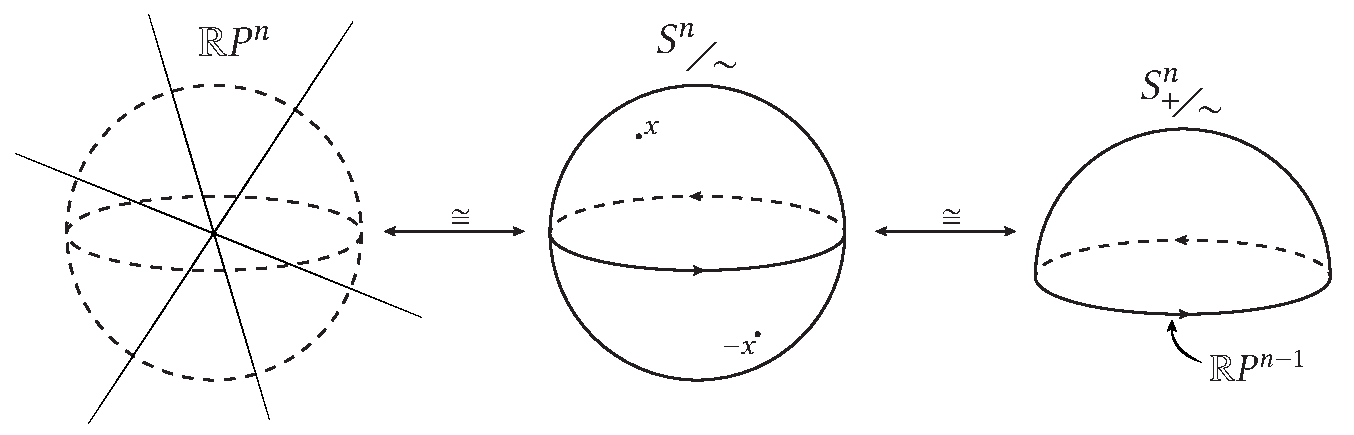
\includegraphics[width=\textwidth]{images/proyecreal.pdf}
\end{figure}
\par 
Así vemos que $\bb{R}P^n = \bb{R}^{n-1} \cup_p e^n$, con $p : S^{n-1} \longrightarrow \bb{R}P^{n-1}$ la proyección. De esta forma $\bb{R}P^n$ admite una estructura con una $i$-celda, $i = 0, 1, \ldots ,n$. \par 
De igual forma $\bb{R}P^\infty = \bigcup_n \bb{R}P^n$ es un CW-complejo con una celda de cada dimensión. 
\end{itemize}
\end{ejems}

\subsection{Construcciones básicas con CW-complejos}
\textbf{Subcomplejos}: Dado un CW-complejo X, un subcomplejo $A$ de $X$ es un subespacio de $X$ obtenido adjuntando celdas de la CW-descomposición y de forma que $A$ sea también CW-complejo. \par
Por ejemplo, el $n$-esqueleto de un complejo es un subcomplejo. O la semiesfera $S_+^n$ es un subcomplejo de $S^n$. \par

\textbf{Productos}:  Si X e Y son CW-complejos (localmente finitos), entonces $X \times Y$ hereda una estructura de CW-complejo donde:
\[ (X \times Y)^n = \bigcup_{i+j=n} X^i \times Y^j \]
Si $e_i$ (resp. $e_j$) es una $i$-celda de $X$ (resp. $j$-celda de $Y$) con $i+j=n$, con aplicación de adjunción $\varphi_i : S^{i-1} \longrightarrow X^{i-1}$ (resp. $\varphi_j : S^{j-1} \longrightarrow X^{j-1}$), consideramos:
\begin{align*} 
e^{i+j} &= e^i \times e^j \text{ donde } \\
S^{n-1} = S^{i+j-1} &= \partial e^{i+j} = \partial e^i \times e^j \ \cup \ e^i \times \partial e^j \\
&= S^{i-1} \times e^j \ \cup \ e^i \times S^{j-1}
\end{align*}

Entonces, $\varphi_i$ y $\varphi_j$ definen $\psi : S^{n-1} \longrightarrow (X \times Y)^{n-1}$ dada por 
\[ \psi = \begin{cases}
\varphi_i  \times \phi_j & \text{ en } S^{i-1} \times e^j \\
\phi_i \times \varphi_j & \text{ en } e^i \times S^{j-1}
\end{cases} \]
donde $\phi_i$ y $\phi_j$ son las aplicaciones características. \par 

\textbf{Cocientes}: Si $(X, A)$ es un CW-par ($A$ es un subcomplejo de $X$) el cociente $\faktor{X}{A}$ hereda de forma natural una estructura de CW-complejo. Las celdas de $\faktor{X}{A}$ son las de $X - A$ más una $0$-celda nueva, la imagen de $A$ en $\faktor{X}{A}$. Para cada $n$-celda $e^n$ en $X - A$ con adjunción $\varphi : S^{n-1} \longrightarrow X^{n-1}$ la correspondiente adjunción en $\faktor{X}{A}$ es $S^{n-1} \longrightarrow X^{n-1} \longrightarrow \faktor{X^{n-1}}{A^{n-1}}$. \par
Por ejemplo, si en $S^{n-1}$ tomamos cualquier CW-estructura y construimos $D^n$ adjuntando una $n$-celda a $S^{n-1}$. $\faktor{D^n}{S^{n-1}} = S^n$ con la estructura usual. Otro ejemplo, si en la superficie $M_g$ de género $g$,  ``colapsamos'' el $1$-esqueleto $\faktor{M_g}{M_g^1} = S^2$. \par 
Nótese también que $\faktor{X^n}{X^{n-1}} = \displaystyle \bigvee_\alpha S_\alpha^n$ con $\alpha$ variando en el número de $n$-celdas. \par 

\textbf{Wedge o suma puntual}: Si $\{X_\alpha \}_{\alpha \in I}$ son CW-complejos y $x_0^\alpha \in X_\alpha$  son $0$-celdas, el wedge $\bigvee_{\alpha \in I} X_\alpha$ obtenido al identificar puntos $\{x_0^\alpha \}$ no es más que el cociente $\faktor{\dot{\cup} X_\alpha}{\{x_0^\alpha\}}$ y tiene por lo anterior estructura de CW-complejo. \par

\textbf{Smash:} El smash de $2$ espacios $X$ e $Y$  se define como $X \wedge Y = \faktor{X \times Y}{X \vee Y}$ entendiendo $X \vee Y = X \times \{y_0\} \cup \{x_0\} \times Y$. \par 
Si $x_0$ e $y_0$ son $0$-celdas de $X$ e $Y$ respectivamente, entonces $X \times \{y_0\} \cup \{x_0\} \times Y$ es un subcomplejo de $X \times Y$ y podemos tomar el cociente considerando la estructura cociente $X \wedge Y$. \\
Por ejemplo, $S^m \wedge S^n = \faktor{S^m \times S^n}{S^m \vee S^n}$ tiene pues una $0$-celda y una $(n+m)$-celda, por lo cual $S^m \wedge S^n = S^{m+n}$. En particular, $S^1 \wedge S^1 = \faktor{T^2}{S^1 \vee S^1} = S^2$: \par 
\begin{figure}[h]
\centering
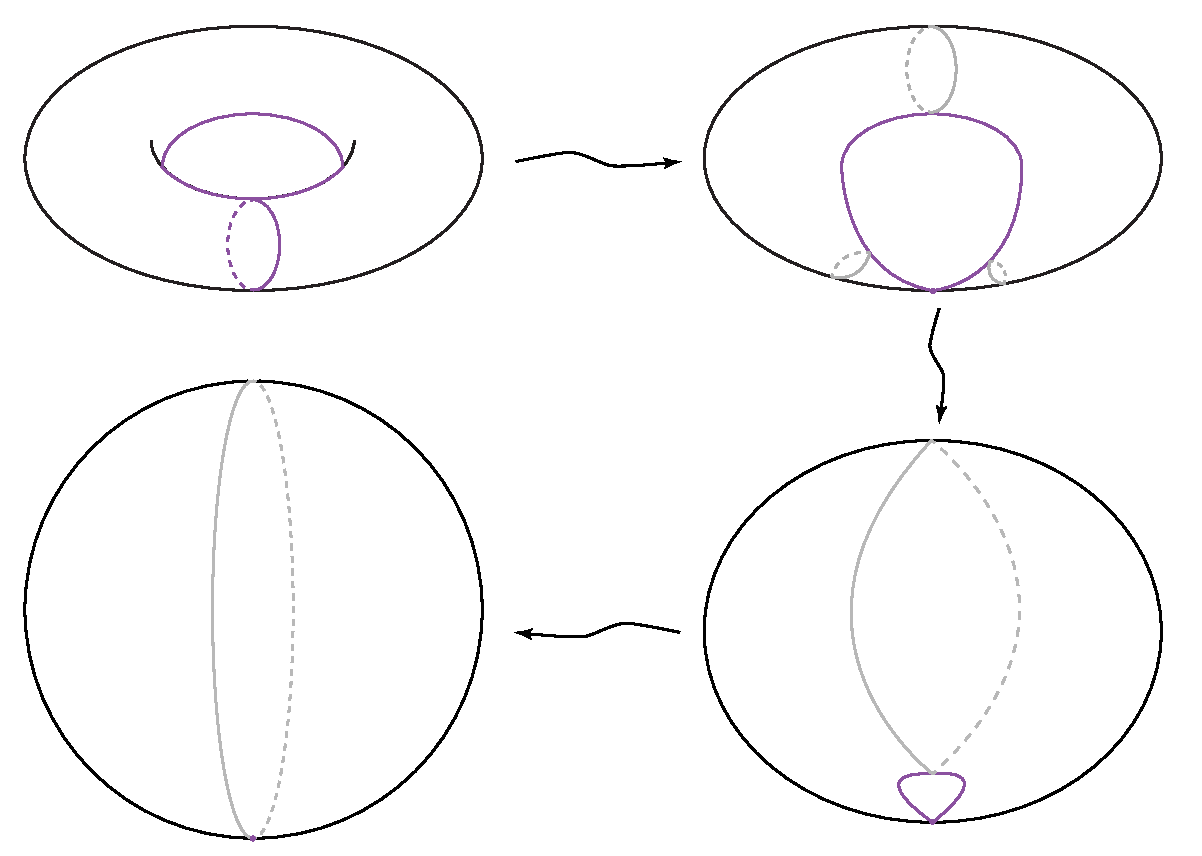
\includegraphics[width = 0.6\linewidth]{images/smashs2}
\end{figure}

\textbf{Espacios de aplicaciones}: SI $X$ es un CW-complejo con finitas celdas e $Y$ tiene un número numerable de ellas, entonces los espacios
$map(X,Y)$, $Y^X$ ó $(Y, y_0)^{(X, \ x_0)}$ tienen el tipo de homotopía de CW-complejos. En los espacios de aplicaciones tomamos siempre la topología compacto abierta, es decir, la que tiene por subbase a los conjuntos 
\[ \langle K, \theta \rangle = \{f:X \longrightarrow Y : f(K) \subset \theta \}, \]
donde $K$ es compacto de $X$ y $\theta$ es abierto de Y.

\section{Suspensión de un espacio y espacio de lazos}
Como ya hemos visto, el \hyperlink{ecom:cono}{cono de $X$}, $CX$, es el espacio contráctil $CX = \faktor{X \times I }{X \times \{ 0 \}}$. De igual forma, la suspensión de $X$, denotada por $\Sigma X$, se define como \par 
\begin{tabular}{ll}
\begin{minipage}{0.5\textwidth}
\[ \Sigma X =  \faktor{X \times I}
{ \footnotesize{\begin{matrix}
(x, 1) \sim (x', 1) \\
(x, 0) \sim (x', 0)
\end{matrix}}} \] 
\end{minipage}
&
\begin{minipage}{0.5\textwidth}
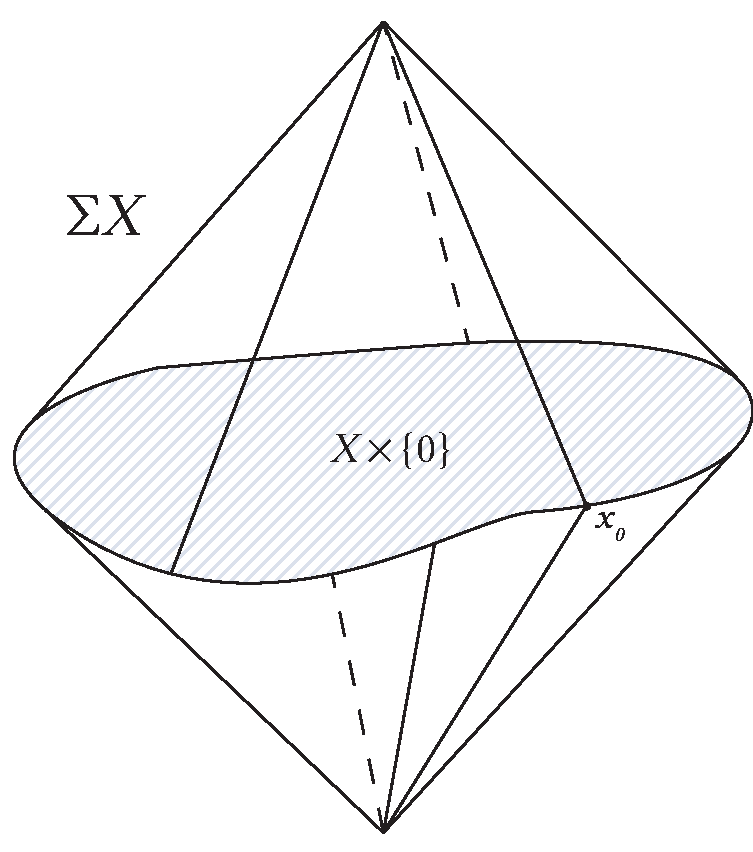
\includegraphics[width=0.6\textwidth]{images/suspensionalt.pdf}
\end{minipage}
\end{tabular}
Si $x_0$ es el punto base de $X$, el cono punteado es
\[ CX = \faktor{X \times I}{X \times \{ 1 \}  \cup \{ x_0 \} \times I}\]
De igual forma la suspensión punteada es 
\[ \Sigma X = \faktor{ X \times I }
{\footnotesize{ \begin{matrix}
(x, 1) \sim (x', 1) \\ 
(x, 0) \sim (x', 0) \\ 
(x_0, t) \sim (x_0, t')
\end{matrix} }} \]
En el caso de que $X$ sea un $CW$-complejo, si a $I$ le damos una  estructura de $CW$-complejo cuya $CW$-descomposición consiste en dos $0$-celdas y una $1$-celda, tanto el cono $CX$ como la suspensión $\Sigma X$ (que no es más que $CX \Bign/ X \times \{ 0 \}$) tienen estructura de $CW$-complejos. \par
Además toda aplicación $f : X \longrightarrow Y$ se puede suspender $\Sigma f : \Sigma X \longrightarrow \Sigma Y$ de forma obvia:
\[\Sigma f [x, t] = [f(x), t]. \]

Por otro lado tenemos los lazos en un espacio topológico punteado $(X, x_0)$ que se definen como
\begin{align*}
\Omega X &= (X, x_0)^{(S^1, \ p_0)} = \{ f : S^1 \longrightarrow X \ \vert \ f(p_0)  = x_0 \} \\ 
&= \{ f : I \longrightarrow X \ \vert \ f(0) = f(1) = x_0 \}
\end{align*}
Se tiene que $\Omega X$ resulta ser $CW$-complejo si $X$ lo es. $\Omega X$ está punteado por la constante en $x_0$, $c_{x_0}$. Se tiene entonces: 
\newpage
\begin{teor}
Para cualesquiera espacios punteados $X$ e  $Y$ se tiene que 
\begin{center}
$[\Sigma X, Y ] \cong [X, \Omega Y]$ \footnote{Siempre que se escriban clases de homotopía, se referirá a clases de homotopía de espacios punteados.}.
\end{center}
\end{teor}
\begin{demo}
En general, veamos que

\[ (Y, y_0)^{(\Sigma X, \ \ast)} \cong (\Omega Y, \ast)^{(X, \ x_0)}. \]

En efecto, la aplicación

\[ \varphi : (\Omega Y, \ast)^{(X, \ x_0)} \longrightarrow (Y, y_0)^{(\Sigma X, \ \ast)}, \]
dada por 
\begin{align*}
\varphi (g) : \Sigma X \longrightarrow Y, \\
\varphi (g)[x, t] = g(x)(t),
\end{align*} 
está bien definida y tiene por inversa a 
\begin{align*}
\varphi^{-1} :  (Y,  y_0)^{(\Sigma X, \ \ast)} \longrightarrow & \ (\Omega Y, \ast)^{(X, \ x_0)},\\
\varphi^{-1} (f) : X \longrightarrow & \ \Omega Y, \\
\varphi^{-1}(f)(x)(t) = & \ f[x, t].
\end{align*}
Veamos que $\varphi$ induce una aplicación $\bar{\varphi} : [X, \Omega Y] \longrightarrow [\Sigma X, Y] $. Hemos de ver que si $f \simeq_{\{ x_0 \}} g$ entonces $\varphi (f) \simeq_{\ast} \varphi (g)$. \par
Sabemos pues que existe una homotopía $H: X \times I \longrightarrow \Omega Y$ tal que $H(x,0) = f(x) $, $H(x,1) = g(x)$ y 
$H(x_0, t) = c_{y_0}$ $\forall t \in I$.\\
Definimos entonces 
\begin{align*}
F: \Sigma X \times I &\longrightarrow Y, \\
F([x,t],s) &= H(x,s)(t), \\
F([x,t],0) &= H(x,0)(t) = f(x)(t) = \varphi(f)[x,t], \\
F([x,t], 1) &= \varphi(g)[x,t], \\
F([x_0,t],s) &= H(x_0, s)(t) = y_0,
\end{align*}
que es una homotopía entre $\varphi (f)$ y $\varphi (g)$.
De igual forma, $\varphi^{-1}$ induce la aplicación $\overline{\varphi^{-1}} : [\Sigma X, Y] \longrightarrow [X, \Omega Y]$ y se tiene que $\overline{\varphi}^{-1} = \overline{\varphi^{-1}}$.\\
\end{demo}

\textbf{Observación:} $\Omega$ y $\Sigma$ son duales en el sentido de Eckmann-Hilton. \par

En $\Omega X$ podemos definir la operación  $\mu : \Omega X \times \Omega X \longrightarrow \Omega X$
\[
\mu(\omega, \omega')(t) = 
\left\{ \begin{array}{ll}
             \omega(2t)		&   $si $ t \leq \frac{1}{2}, \\
             \omega'(2t-1)	&   $si $ t \geq \frac{1}{2}. \\
        \end{array}
\right.
\]
$\mu(\omega, \omega')$ está bien definida y para ver que es continua basta observar que la aplicación
\begin{align*}
\Omega X \times \Omega X \times I &\longrightarrow \Omega X \times I \longrightarrow X, \\
(\omega, \omega', t) &\longmapsto 
\left\{ \begin{array}{ll}
             \omega(2t)		&  t \leq \frac{1}{2}, \\
             \omega'(2t-1)	&  t \geq \frac{1}{2}, \\
        \end{array}
\right.
\end{align*}
 es continua. \\
Esta operación permite definir otra en $[X, \Omega Y]$, dada por 
\[  
[f] \cdotp [g] = [\mu(f, g)] 
\]

Veamos que $\mu$ hace de $\Omega Y$ un grupo homotópico, esto es, un grupo en la categoría homotópica de los espacios topológicos. Demostremos la siguiente proposición:
\begin{prop}
Sea $(Y, y_0)$ un espacio topológico punteado. Consideremos el espacio de lazos $\Omega Y$. Entonces
\begin{enumerate}
\item $c_{y_0}$ es el neutro homotópico.
\item $\mu$ es homotópicamente asociativa.
\item Si $\omega \in \Omega Y$, entonces el inverso homotópico de $\omega$ es $\omega^{-1}(t) = \omega(1 - t)$.
\end{enumerate}
\end{prop}
\begin{demo}
\begin{enumerate}
\item Veamos que $c_{y_0}$ es neutro por la derecha. Consideramos
\begin{align*}
\mu(-,c_{y_0}) : \Omega Y &\longrightarrow \Omega Y, \\
\omega &\longmapsto \omega \cdotp c_{y_0}.
\end{align*}
Tenemos que ver que es homótopa a la identidad. Para ello basta considerar la homotopía
\begin{align*}
F&: \Omega Y \times I \longrightarrow \Omega Y, \\
F(\omega, t)(s) &= 
\begin{cases}
\omega\left(\frac{2s}{t+1}\right) & 0 \leq s \leq \frac{t+1}{2}, \\
y_0													& \frac{t+1}{2} \leq s \leq 1.
\end{cases}
\end{align*}
Igualmente se demuestra que $\mu(c_{y_0}, -) \simeq Id_{\Omega Y}$.
\item Para ver que $\mu$ es asociativa, tenemos que ver que el siguiente diagrama es homotópicamente conmutativo: 
\[
\begin{tikzcd}
	\Omega Y \times \Omega Y \times \Omega Y \rar{\mu \times Id_{\Omega Y}} \dar{Id_{\Omega Y} \times \mu}
		  & \Omega Y \times \Omega Y \dar{\mu} \\
	\Omega Y \times \Omega Y \rar{\mu} 
		  & \Omega Y \ .
\end{tikzcd}
\]
La homotopía necesaria para esto es:
\begin{align*}
G: 	\Omega Y &\times \Omega Y \times \Omega Y \times I \longrightarrow \Omega Y, \\
G(\omega, \omega' \omega'', t)(s) &= 
\begin{cases}
\omega \left( \frac{4s}{t+1}\right) & 0 \leq s \leq \frac{t+1}{4}, \\
\omega'(4s - t - 1)         		 & \frac{t+1}{4} \leq s \leq \frac{t+2}{2}, \\
\omega''\left( \frac{4s -2 - t}{2-t}\right) & \frac{t+2}{4} \leq s \leq 1.
\end{cases}
\end{align*}

\item Por último, definimos el morfismo inverso $\varPhi : \Omega Y \longrightarrow \Omega Y $ dado por $\varPhi(\omega) = \omega^{-1}$. Tenemos que ver que $\omega \cdotp \omega^{-1} \simeq c_{y_0}$. Para ello consideramos la homotopía:
\begin{align*}
H &: \Omega Y \times I \longrightarrow \Omega Y, \\
H(\omega, t)(s) &= 
\begin{cases}
y_0 & 0 \leq s \leq \frac{t}{2}, \\
\omega(2s - t) & \frac{t}{2} \leq s \leq \frac{1}{2}, \\
\omega(2 - 2s - t) & \frac{1}{2} \leq s \leq 1 - \frac{t}{2}, \\
y_0 & 1 - \frac{t}{2} \leq s \leq 1.
\end{cases}
\end{align*}
\end{enumerate}
\end{demo}
Vista esta proposición, de forma inmediata se tiene que:
\begin{teorf}
$[X, \Omega Y]$ es un grupo.
\end{teorf}
Este proceso que hemos seguido puede realizarse de forma dual para la suspensión $\Sigma X$:\par
En la suspensión de un espacio existe una co-operación natural
\begin{align*}
\Sigma X &\stackrel{\nu}{\longrightarrow} \Sigma X \vee \Sigma X, \\
\nu [x, t] &= 
\begin{cases}
([x, 2t], \ast ) & t \leq \frac{1}{2}, \\
( \ast, [x, 2t -1]) & t \geq \frac{1}{2}.
\end{cases}
\end{align*}
\begin{figure}[h]
\centering
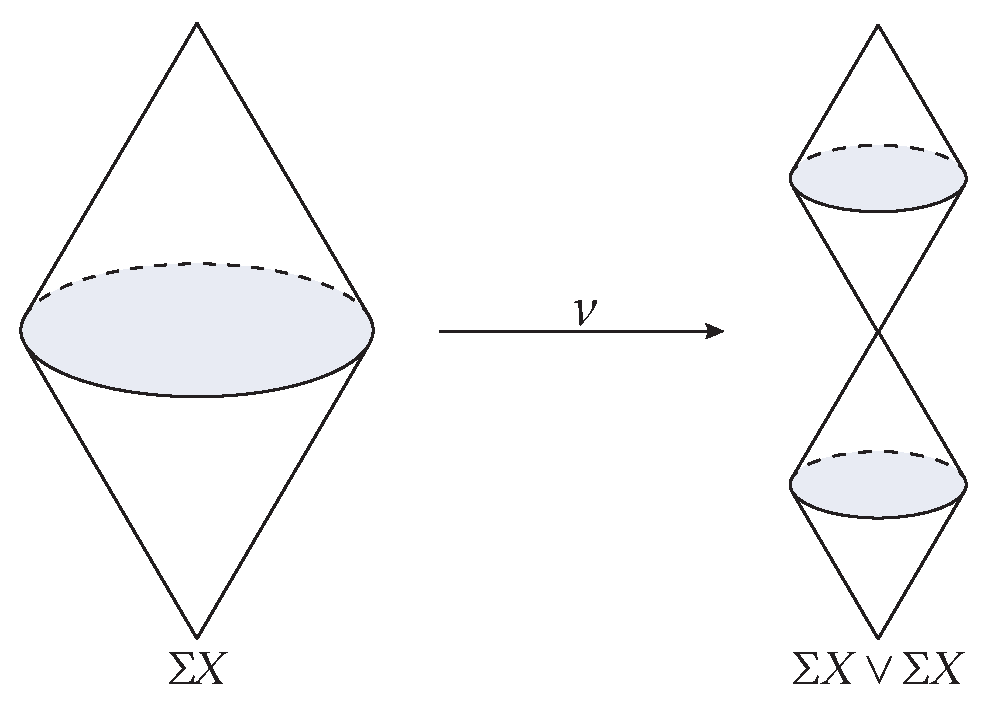
\includegraphics[width=0.45\textwidth]{images/suspoperac.pdf}
\end{figure}

\par
que resulta ser co-asociativa con co-elemento neutro y con co-elemento inverso homotópico:
\begin{prop}
\begin{enumerate}
\item Asociatividad:
\begin{tikzcd}
	\Sigma X \rar{\nu} \dar{\nu} & \Sigma X \vee \Sigma X \dar{1 \vee \nu} \\
	\Sigma X \vee \Sigma X \rar{\nu \vee 1} & \Sigma X \vee \Sigma X \vee \Sigma X.
\end{tikzcd}
\item Elemento neutro:
\begin{tikzcd}
	\Sigma X \rar{\nu} \arrow[bend right = 20]{rrr}{1}
 		& \Sigma X \vee \Sigma X \rar{c_{x_0} \vee 1} & \Sigma X \vee \Sigma X \rar{\sigma} & \Sigma X.
\end{tikzcd}
\item Elemento inverso:
\begin{tikzcd}
	\Sigma X \rar{\nu} \arrow[bend right = 20]{rrr}{c_{x_0}}
		& \Sigma X \vee \Sigma X \rar{1 \vee \eta} & \Sigma X \vee \Sigma X \rar{\sigma} & \Sigma X,
\end{tikzcd} \\
donde $\eta : \Sigma X \longrightarrow \Sigma X \text{,	} \eta[x,t] = [x, 1-t]$.
\end{enumerate}
\end{prop}
Esta co-operación define en $[\Sigma X, Y]$ una operación
\[
\begin{tikzcd}
\Sigma X \rar{\nu} & \Sigma X \vee \Sigma X \rar{f \vee g} & Y \vee Y \rar{\sigma} & Y
\end{tikzcd}
\]
que por la proposición anterior implica:
\begin{teorf}
$[\Sigma X, Y]$ es un grupo.
\end{teorf}
Es fácil ver el siguiente resultado.
\begin{teor}
La aplicación $\bar{\varphi} : [\Sigma X, Y] \longrightarrow [X, \Omega Y]$
es un isomorfismo de grupos.
\end{teor}

\subsection{Caso particular grupos de homotopía: $X = S^n$}
Como ya definiremos con más detalle en el capítulo 4, se define el grupo de homotopía n-ésimo relativo al punto base $x_0$ como 
\[ \homot{n}{X, x_0} = [(I^n, \partial I^n), (X, x_0)]. \]
Las aplicaciones $(I^n, \partial I^n) \longrightarrow (X, x_0)$ pueden verse como aplicaciones 
\[(S^n, p_0) \longrightarrow (X, x_0) \] 
ya que $\faktor{I^n}{\partial I^n} = S^n$ y $\faktor{\partial I^n}{\partial I^n} = p_0$. \par
De esta forma, el grupo de homotopía $n$-ésimo es:
\[ \pi_n(X, x_0) = [S^n, X]. \]

La operación interna de este grupo se ve muy bien de forma geométrica en esta interpretación del grupo de homotopía: \par
\begin{figure}[h]
\centering
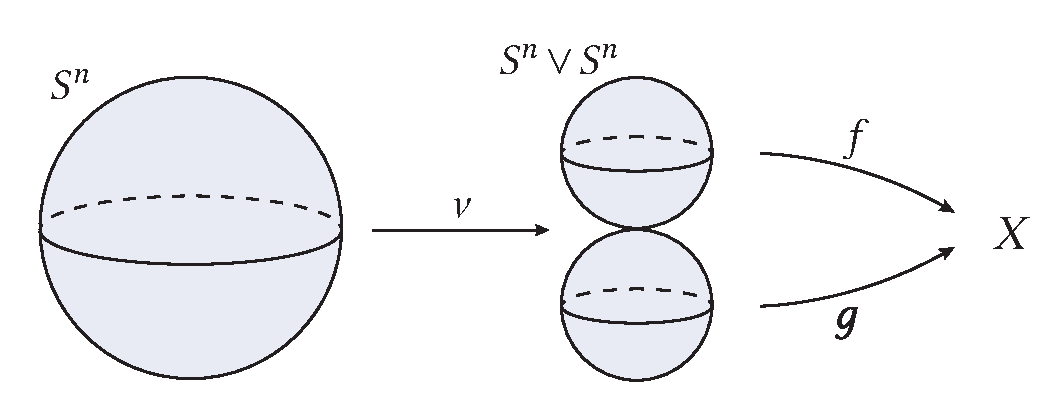
\includegraphics[width=0.7\textwidth]{images/ejgruphomot.pdf}
\end{figure}

Ahora bien, teniendo en cuenta que $\Sigma S^n = S^{n+1} \ \forall n \geq 0$, y el teorema anterior, tenemos el siguiente resultado:
\begin{teorf}
$\pi_n(X) = [S^n, X] = [S^{n-1}, \Omega X] = \pi_{n-1}(\Omega X)$.
\end{teorf}
\newpage
\mbox{}
\thispagestyle{plain}